\documentclass{beamer}
%
% Choose how your presentation looks.
%
% For more themes, color themes and font themes, see:
% http://deic.uab.es/~iblanes/beamer_gallery/index_by_theme.html
%
\mode<presentation>
{
  \usetheme{Warsaw}      % or try Darmstadt, Madrid, Warsaw, ...
  \usecolortheme{default}
  \usepackage{beamerthemesplit}% or try albatross, beaver, crane, ...
  \usefonttheme{default}  % or try serif, structurebold, ...
  \setbeamertemplate{navigation symbols}{}
  \setbeamertemplate{caption}[numbered]
  \setbeamertemplate{headline}{}
  \AtBeginSection[]{
    \begin{frame}
    \vfill
    \centering
    \begin{beamercolorbox}[sep=8pt,center,shadow=true,rounded=true]{title}
      \usebeamerfont{title}\insertsectionhead\par%
    \end{beamercolorbox}
    \vfill
    \end{frame}
  }
  \AtBeginSubsection[]{
    \begin{frame}
    \vfill
    \centering
    \begin{beamercolorbox}[sep=8pt,center,shadow=true,rounded=true]{title}
      \usebeamerfont{title}\insertsubsectionhead\par%
    \end{beamercolorbox}
    \vfill
    \end{frame}
  }
}
\usepackage[english,russian]{babel}
\usepackage[utf8]{inputenc}
\usepackage{amsmath}
\usepackage{dutchcal} %math symbols
\usepackage{hyperref}
\usepackage[backend=bibtex]{biblatex}
\bibliography{bibliography.bib}

% Removes icon in bibliography
\setbeamertemplate{bibliography item}{}

\hypersetup{unicode=true}

\title[Обзор литературы по ассембелрам]{Обзор литературы по ассембелрам}
\author{Дмитрий Яковлев}
\institute{EPAM Systems}
\date{\today}

\begin{document}
\graphicspath{{./img/}}

\begin{frame}
  \titlepage
\end{frame}

\begin{frame}
\frametitle{План}
\tableofcontents
\end{frame}

\section{Ввведение}
% !TEX root = ../review.tex
\begin{frame}

\begin{center}

\end{center}

\end{frame}


\section{Модель ошибки на данных BioNano}
% !TEX root = ../review.tex
\begin{frame}
\frametitle{Модель ошибок: общие сведения}
\begin{itemize}
  \item Было рассмотрено 3 датасета карт от BioNano
  \item С помощью RefAligner был построен референс
  \item Далее был проведён анализ ошибок
\end{itemize}
\end{frame}

\begin{frame}
\frametitle{Модель ошибок: ошибка в длине фрагмента}


\begin{figure}
\centering
\begin{minipage}{.5\textwidth}
  Валуев:
  \begin{gather*}
  e_k = \frac{o_k - r_k}{\sqrt{r_k}} \sim N(0, \sigma) \\
  o_k \sim N(r_k, \sigma^2 \, r_k)
  \end{gather*}
  \centering
  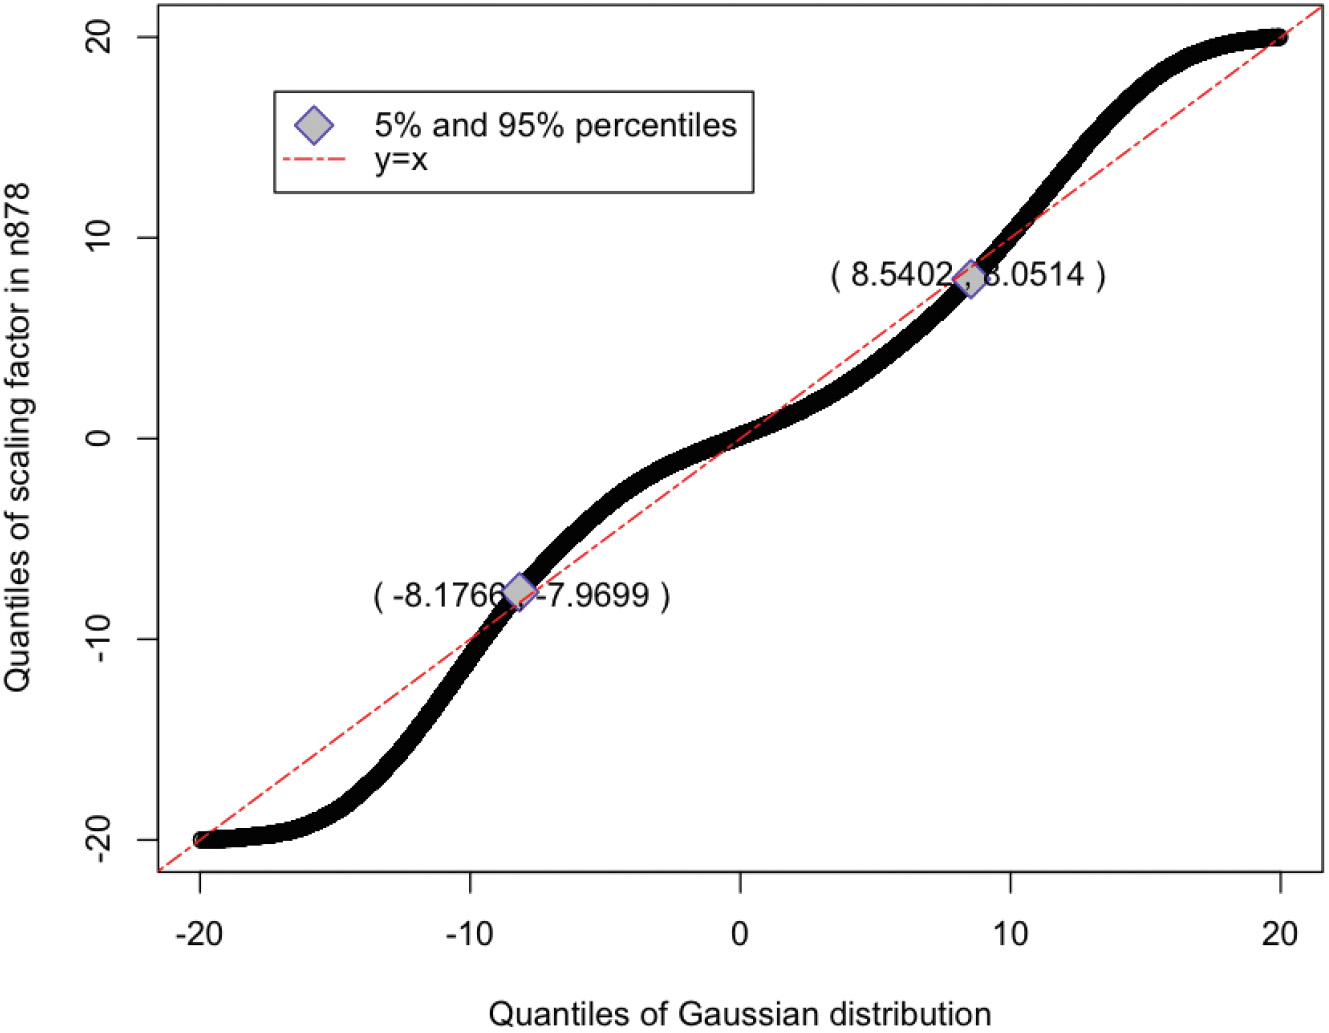
\includegraphics[width=.9\linewidth]{error_model/sigma_error_norm}
\end{minipage}%
\begin{minipage}{.5\textwidth}
  Новый подход:
  \begin{gather*}
  s_k = \frac{o_k}{r_k} \\
  s_k \sim Laplace(\mu, \beta)
  \end{gather*}
  \centering
  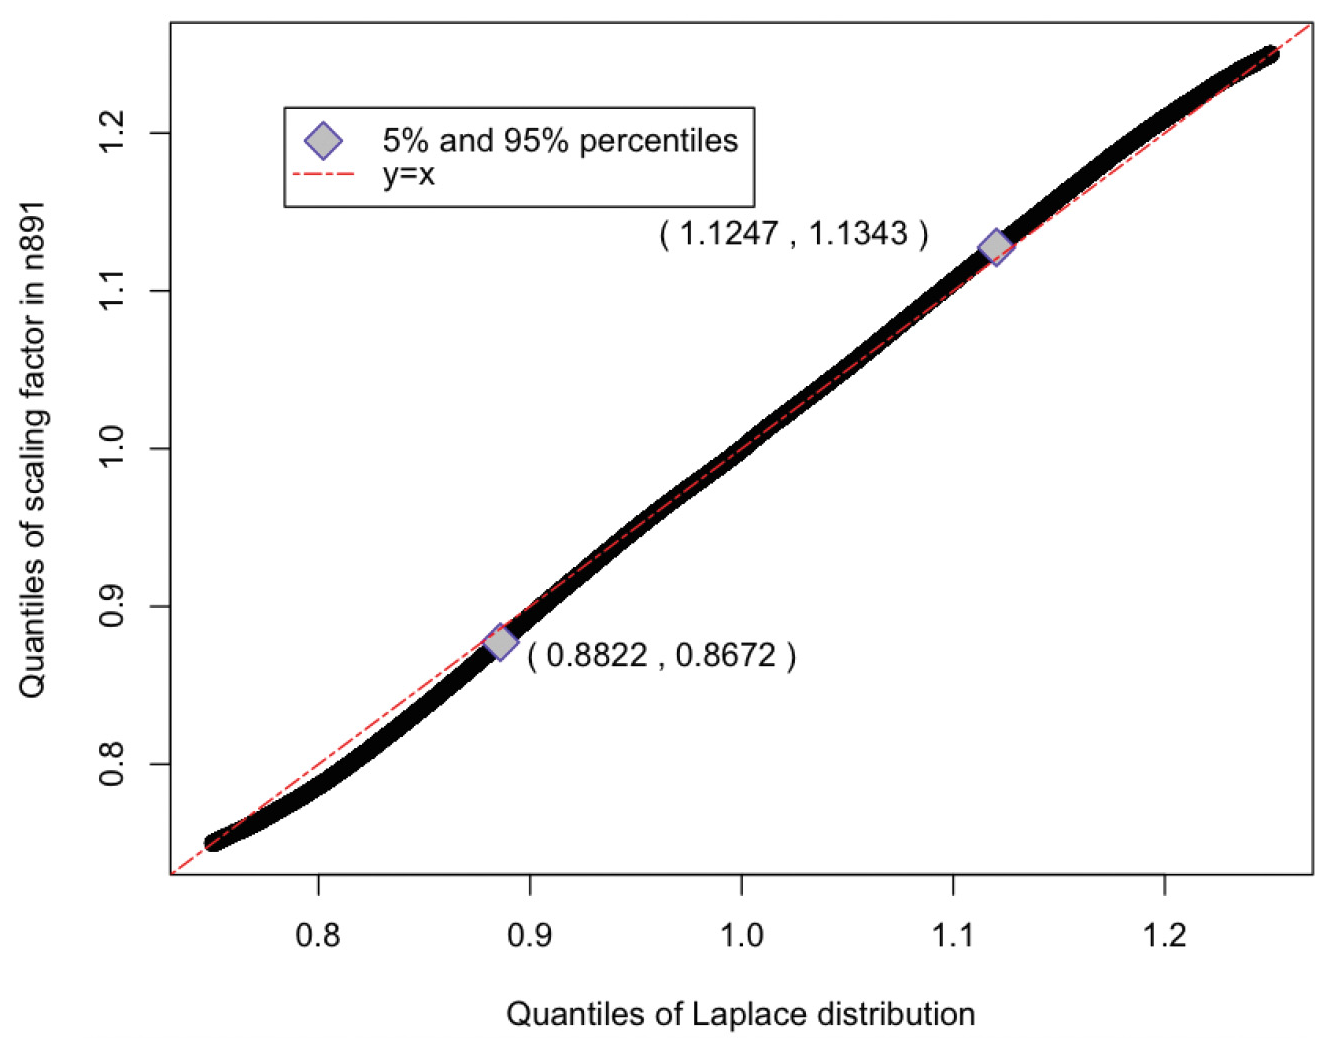
\includegraphics[width=.9\linewidth]{error_model/sigma_error_laplace}
\end{minipage}
\end{figure}
\end{frame}

\begin{frame}
\frametitle{Модель ошибок: пропущенные разрезы}
Было замечено, что вероятность пропущенного разреза зависит от длины до соседних разрезов.
\begin{figure}
  \centering
  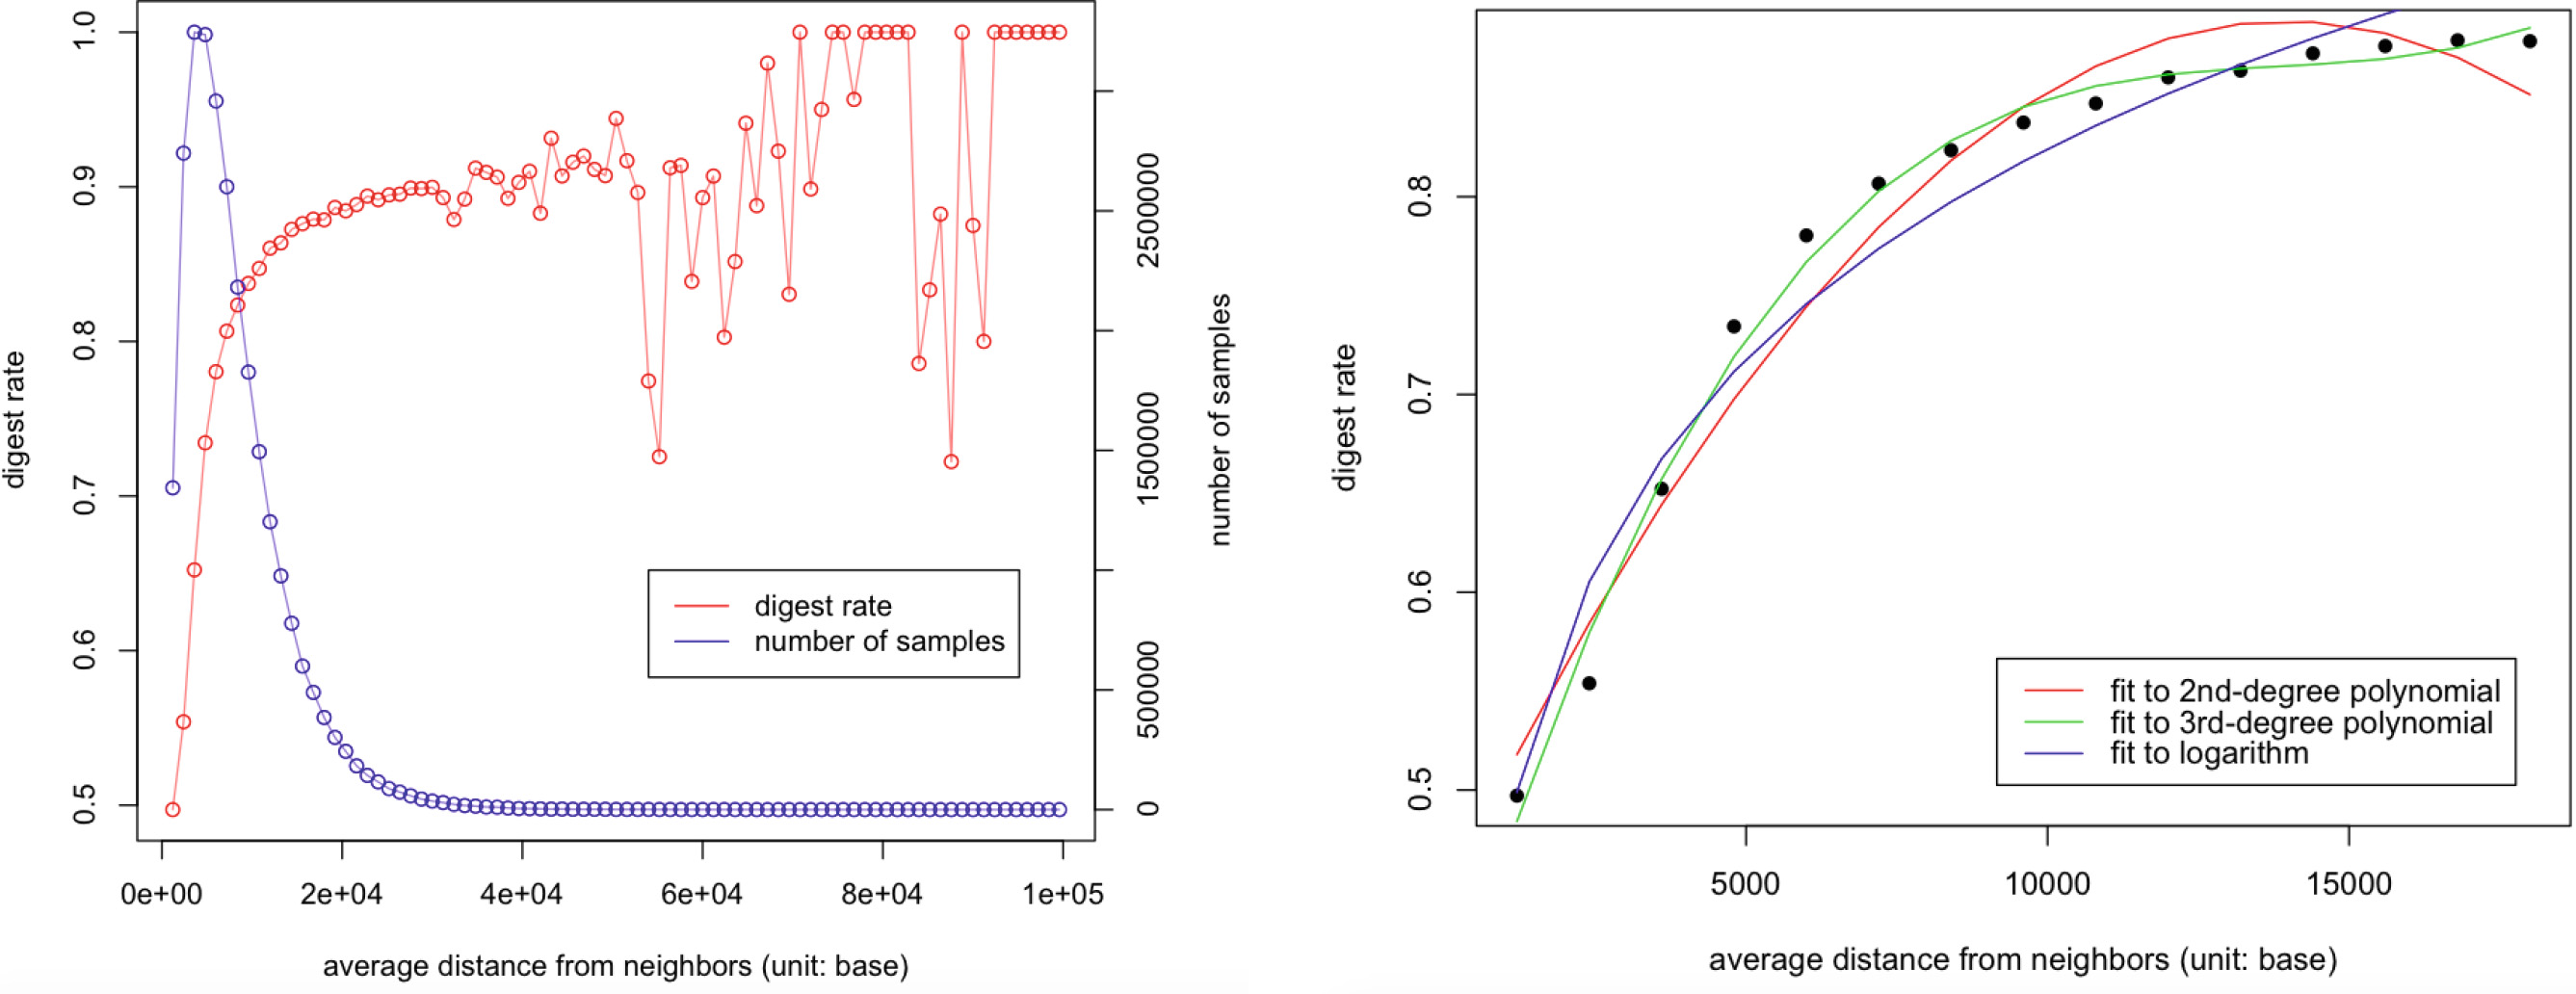
\includegraphics[width = 0.9\textwidth]{error_model/pc_error}
\end{figure}
\begin{gather*}
p_c (d_{avg}) = \alpha_3 \, d_{avg}^3 + \alpha_2 \, d_{avg}^2 +  \alpha_1 \, d_{avg} + \alpha_0 \\
d_{avg} = \frac{\text{среднее расстояние до соседей}}{1200}
\end{gather*}
\end{frame}

\begin{frame}
\frametitle{Модель ошибок: лишние разрезы (1)}
\begin{figure}
  \centering
  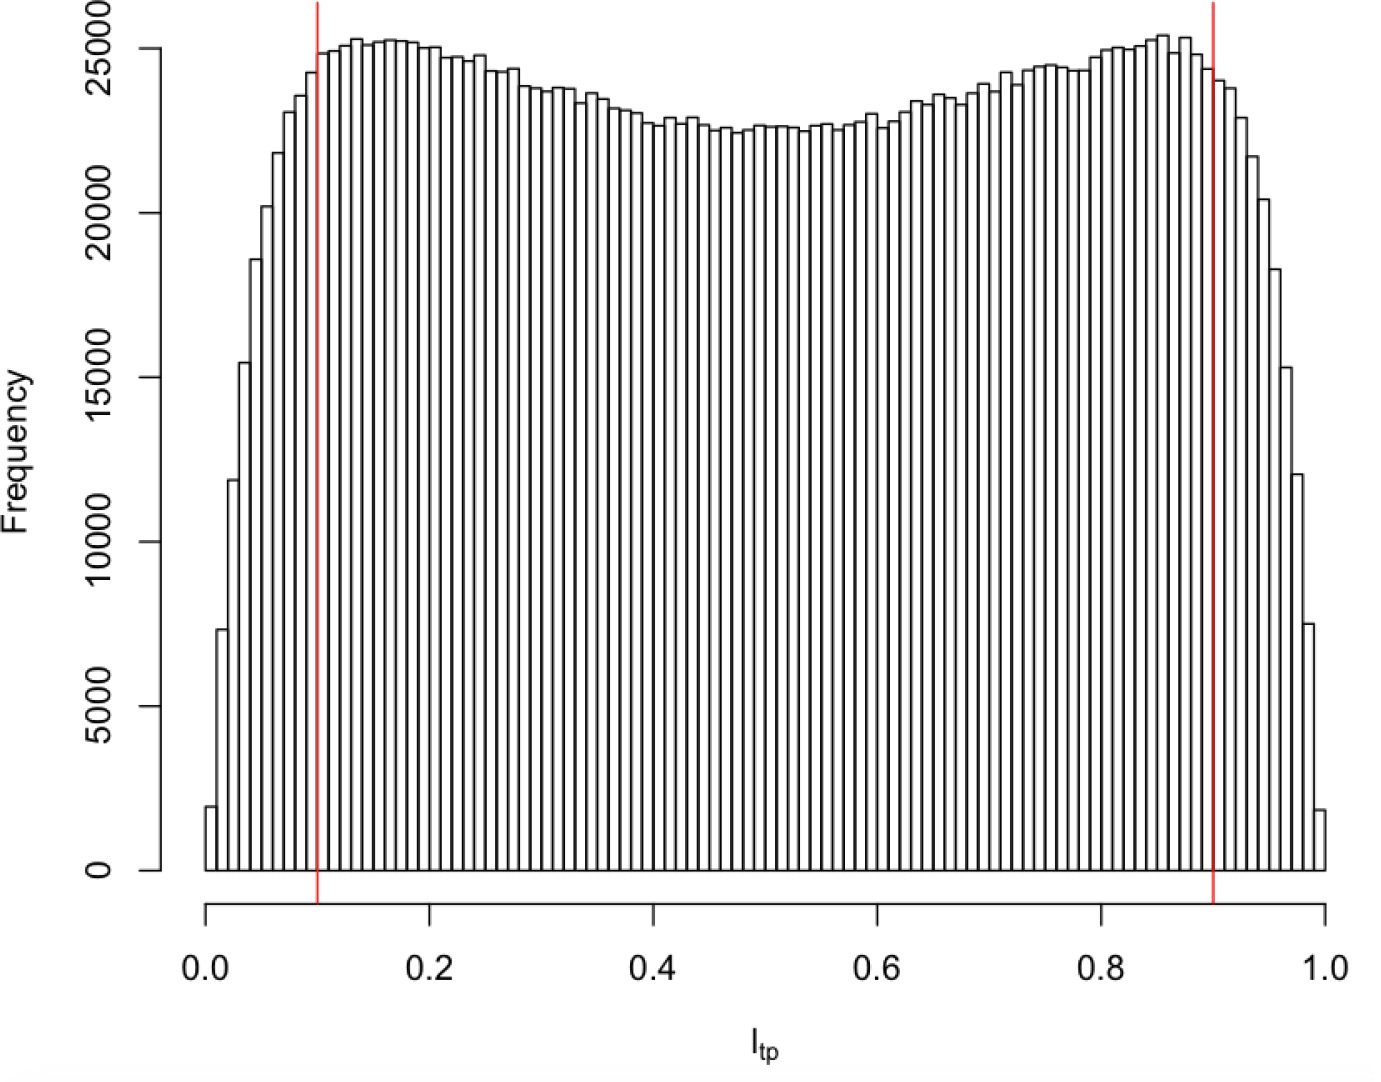
\includegraphics[width = 0.9\textwidth, height = 0.6\textheight]{error_model/false_cut_error_loc}
\end{figure}
\begin{gather*}
l_{fp} = \frac{\text{расстояние от лишнего разреза до конца карты}}{\text{длина оптической карты}} \\
n_{fp} \sim 0.18\, Poisson(0) + 0.6 \, Poisson(1) + 0.22 \, Poisson(3)
\end{gather*}

\end{frame}

\begin{frame}
\frametitle{Модель ошибок: лишние разрезы (2)}
\begin{figure}
  \centering
  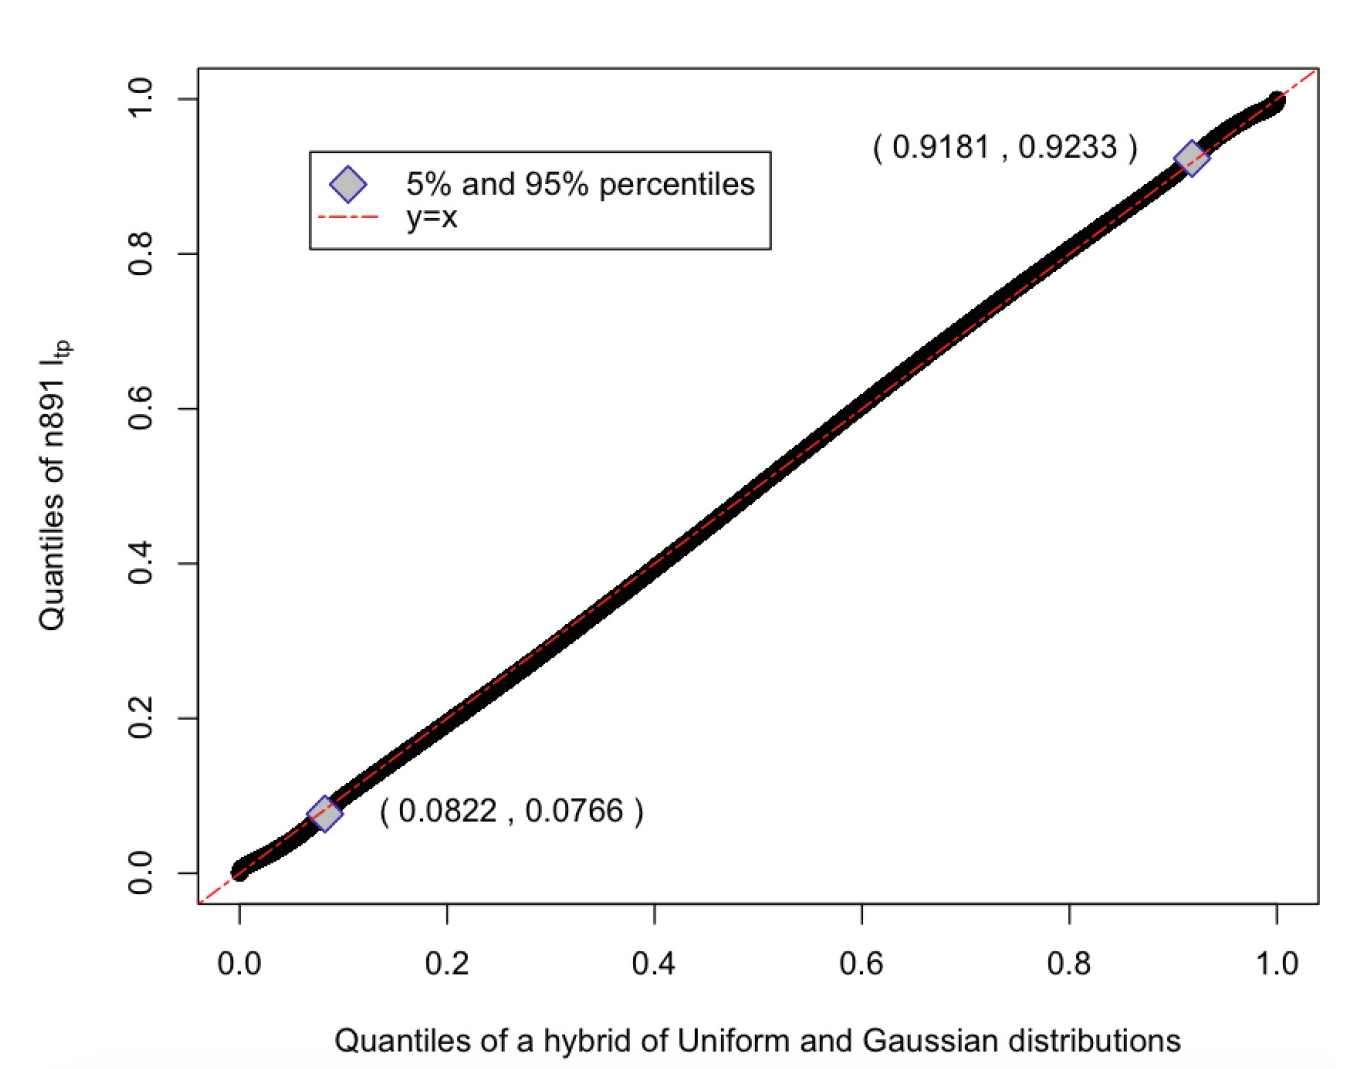
\includegraphics[width = 0.9\textwidth, height = 0.6\textheight]{error_model/false_cut_error}
\end{figure}
\begin{figure}
  \centering
  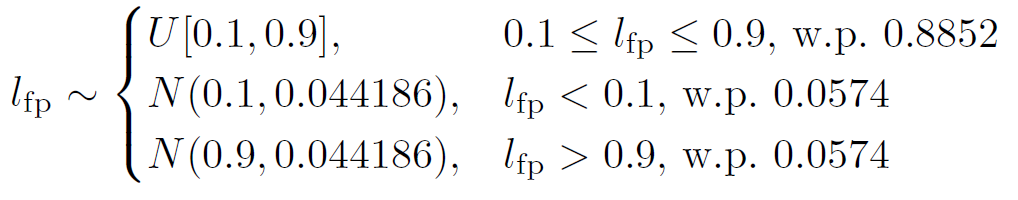
\includegraphics[width = 0.9\textwidth]{error_model/false_cut_solution}
\end{figure}
\end{frame}


\section{Ассемблеры}

\subsection{TWIN}
% !TEX root = ../review.tex

\begin{frame}
\frametitle{TWIN\nocite{twin}: Алгоритм}
Алгоритм разработан в предположении отсутствия пропущенных и лишних разрезов.
Идея:
\begin{itemize}
  \item Построение FM-индекса на референсе
  \item Выравнивание карты на референсе будем искать как подстроку в строке
  \item В статье предлагается алгоритм неточного поиска подстроки в строке
\end{itemize}


\end{frame}


\subsection{OPTIMA}
% !TEX root = ../review.tex
\begin{frame}
\frametitle{OPTIMA: Общие сведения}


\end{frame}

\begin{frame}
\frametitle{OPTIMA: Алгоритм}

Этапы выравнивания:
\begin{itemize}
  \item Поиск стартовых мест (сидов) для начала выравнивания
  \item Парное выравнивание карты с референсом
  \item Определение значимых выравниваний
  \item Объединение пересекающихся выравниваний
\end{itemize}

\end{frame}


\begin{frame}
\frametitle{OPTIMA: Определение значимости выравнивания}
Пусть $a$ - выравнивание из множества выравниваний $\mathcal{A}$
\begin{gather*}
Z-score(a \in \mathcal{A}, f) = \frac{f_{a} - Mean(f_{\mathcal{A}})}{SD(f_{\mathcal{A}})}
\end{gather*}
где $f$ - характеристика выравнивания.\\
 Тогда статистическая значимость выравнивания:
\begin{align*}
  \vartheta (a \in \mathcal{A}) = Z-score( & -Z-score(a, \#matches) \\
  & + Z-score(a, \#cuterrors) \\
  & + Z-score(a, WHT(\chi^2, \#matches))) \\
\end{align*}
\[\text{где } WHT(\chi^2, \#matches) = \frac{\sqrt[3]{\frac{\chi^2}{\#matches}} - \big(1 - \frac{1}{9} \frac{2}{\#matches}\big)}{\sqrt{\frac{1}{9} \frac{2}{\#matches}}}\]
\end{frame}


\subsection{MAligner}
% !TEX root = ../review.tex
\begin{frame}
\frametitle{MAligner\nocite{maligner}: Общие сведения}
Два подхода:
\begin{enumerate}
  \item На основе алгоритма Смита-Ватермана
  \begin{itemize}
    \item Построение множества выравниваний на референсе
    \item Определение значимых выравниваний - M-Score
  \end{itemize}
  \item На основе индексации
\end{enumerate}
\end{frame}

\begin{frame}
\frametitle{MAligner: Алгоритм динамического программирования}

Пусть имеются два выравненных участка c n и m пропущенными фрагментами длины r и m на референсе и карте соотвественно.
Тогда выравнивание имеет следующее значение:

\begin{gather*}
Score(q, r, m, n) = S(q, r) + C_q \,m + C_r \, n \\
S(q, r) = \bigg(\frac{q - r}{\sigma(r)}\bigg)^2 \\
\sigma(r) = \max(\alpha \, r, \sigma_{min})
\end{gather*}
$C_q$ - штраф за пропущенные фрагменты на карте \\
$C_r$ - штраф за пропущенные фрагменты на референсе \\
$\sigma_{min}$ - для фрагментов малой длины, ошибка больше \\
$\alpha$ - доля референса, которая будет использовать как стандартное отклонение
\end{frame}

\begin{frame}
\frametitle{MAligner: M-Score - значимость выравнивания}

Предложена оценка M-Score для определения значимости выравнивания:

\begin{gather*}
  m_{\mathcal{A}} = \underset{A \in \mathcal{A}}{median}\{Score(A)\} \\
  MAD_{\mathcal{A}} = \underset{A \in \mathcal{A}}{median}\{ | Score(A) - m_{\mathcal{A}}|\} \\
  M-Score_{\mathcal{A}}(A) = \frac{Score(A) - m_{\mathcal{A}}}{MAD_{\mathcal{A}}}
\end{gather*}

$Score(A)$ - значение выравнивания $A$

$\mathcal{A}$ - 100 лучших выравниваний по Score(A)
\end{frame}


\begin{frame}
\frametitle{MAligner: Алгоритм на основе индексов}
Работает в предположении, что в карте не могут быть пропущенные разрезы:
\begin{enumerate}
  \item Выбирается k и строятся всевозможные k-tuple на референсе длины меньше k - $\mathcal{K}$ и сортируем его по длине.
  \item Далее строится по множеству $\mathcal{K}$ граф, где вершины - k-tuple, а рёбрами соединяем те k-tuple, у которых граничные разрезы совпадают.
  \item У входной карты берём k-tuple и бинарным поиском по длине в $\mathcal{K}$ ищем схожие k-tuple.
  \item Для каждого найденного k-tuple  запускаем поиск в ширину по графу, при чём идём только по тем вершинам, длины которых $C$ удовлетворяют очередному фрагменту карты длины $c_q$:
  \begin{gather*}
     c_q - max(\alpha \, c_q, \beta) \le C \le c_q + max(\alpha \, c_q, \beta)
  \end{gather*}
  \item Получаем набор выравниваний.
\end{enumerate}
\end{frame}

\begin{frame}
\frametitle{MAligner: Результаты}
  Данные без ошибок:
  \begin{figure}
    \centering
    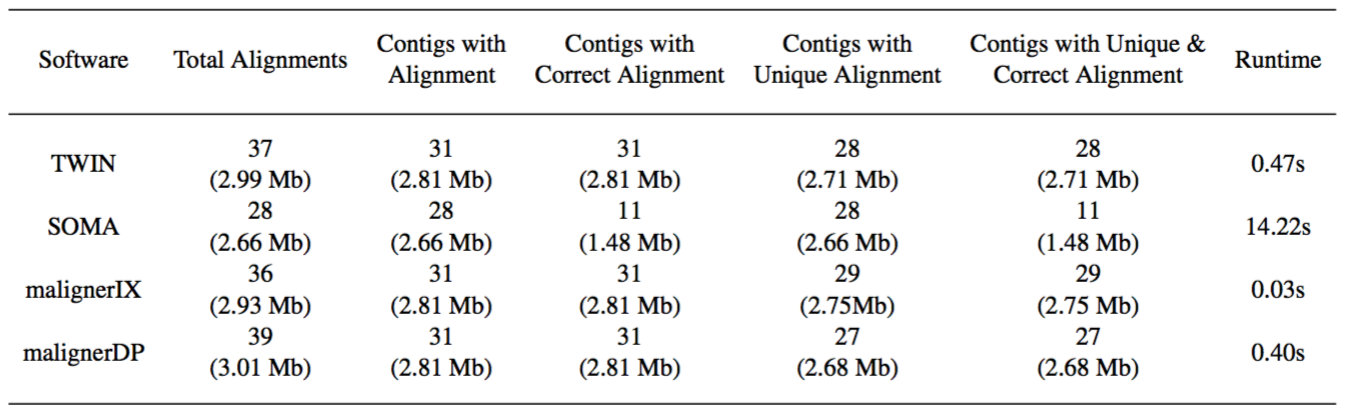
\includegraphics[width = 0.9\textwidth]{maligner/without_errors}
  \end{figure}
  Данные с ошибками:
  \begin{figure}
    \centering
    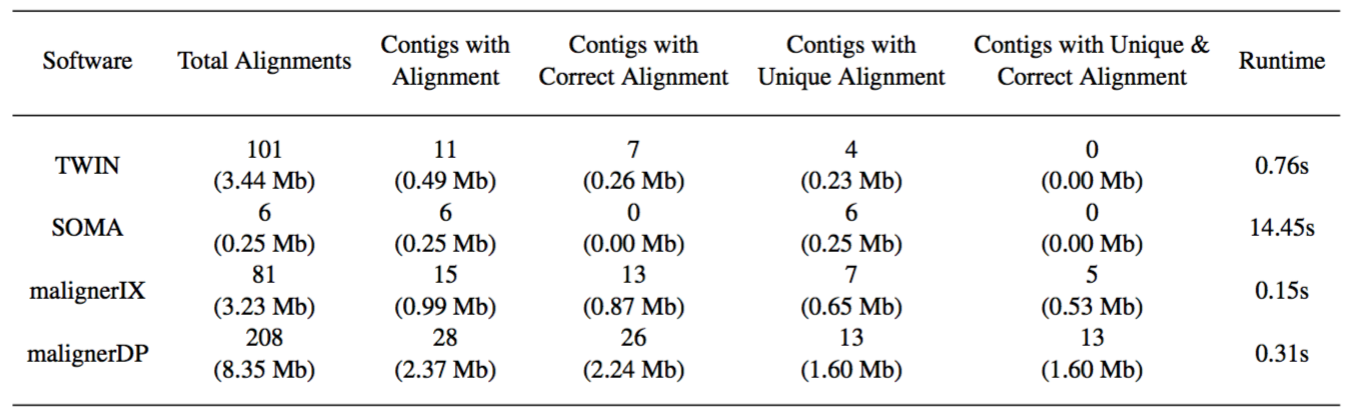
\includegraphics[width = 0.9\textwidth]{maligner/with_errors}
  \end{figure}

\end{frame}


\subsection{OMBlast}
% !TEX root = ../review.tex
% \begin{frame}
% \frametitle{OMBlast\nocite{omblast}: Общие сведения}

% \end{frame}

\begin{frame}
\frametitle{OMBlast\nocite{omblast}: Алгоритм}

Этапы выравнивания:
\begin{itemize}
  \item Поиск стартовых мест (сидов) для начала выравнивания
  \item Расширение сидов
  \item Объединение пересекающих выравниваний
  \item Построение итогового выравнивания
\end{itemize}

\end{frame}

\begin{frame}
\frametitle{OMBlast: Поиск стартовых сидов - индексация}
  Фрагмент $q$ на карте совпадает с фрагментом $r$ на референсе:
  \begin{equation*}
    r(1 - T_s) - T_m \le q \le r(1 + T_s) + T_m
  \end{equation*}
  $T_s$ - параметр, ошибка масштабирования \\
  $T_m$ - параметр, ошибка измерений \\
  \begin{figure}
    \centering
    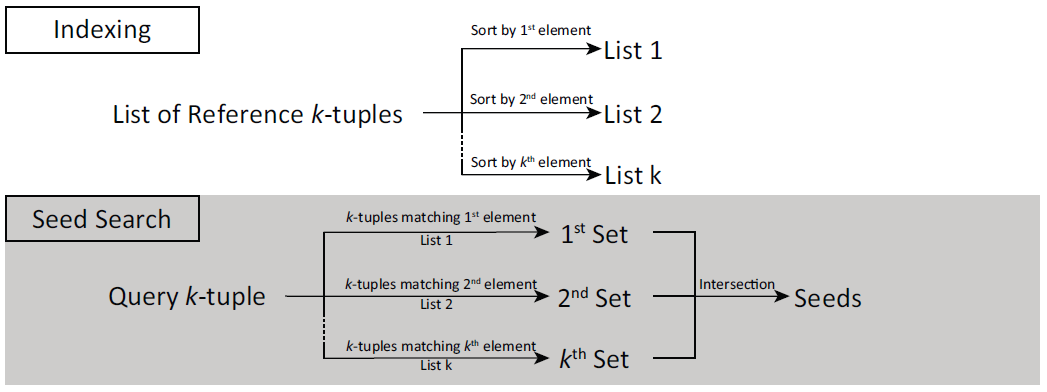
\includegraphics[width = 0.9\textwidth]{omblast/index_A}
  \end{figure}
\end{frame}

\begin{frame}
\frametitle{OMBlast: Поиск стартовых сидов - бины}
  \begin{figure}
    \centering
    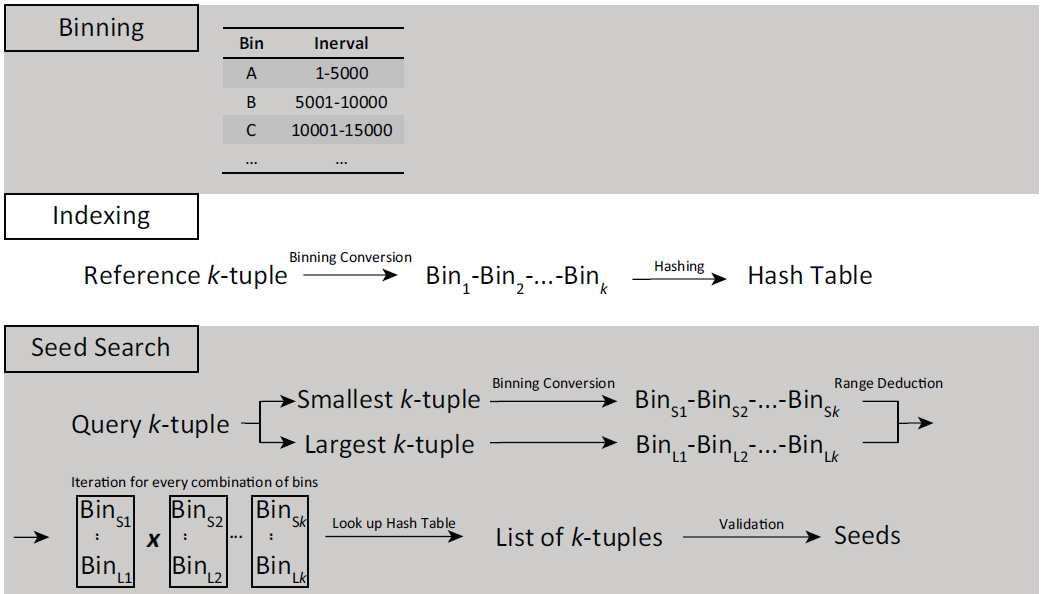
\includegraphics[width = 0.9\textwidth]{omblast/index_B}
  \end{figure}
\end{frame}

\begin{frame}
\frametitle{OMBlast: Расширение сидов}
  \begin{figure}
    \centering
    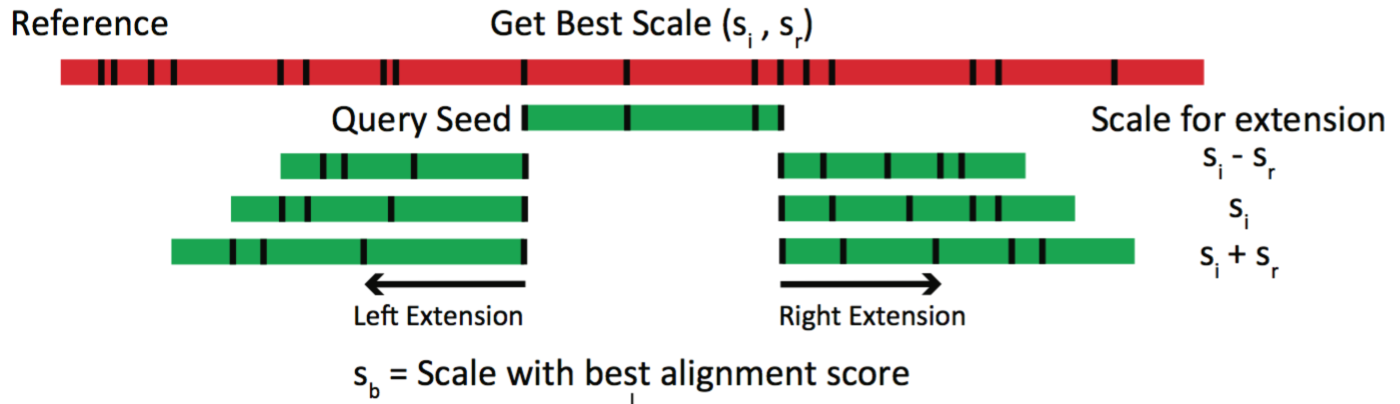
\includegraphics[width = 0.9\textwidth]{omblast/ext_seeds_1}
  \end{figure}
  \begin{figure}
    \centering
    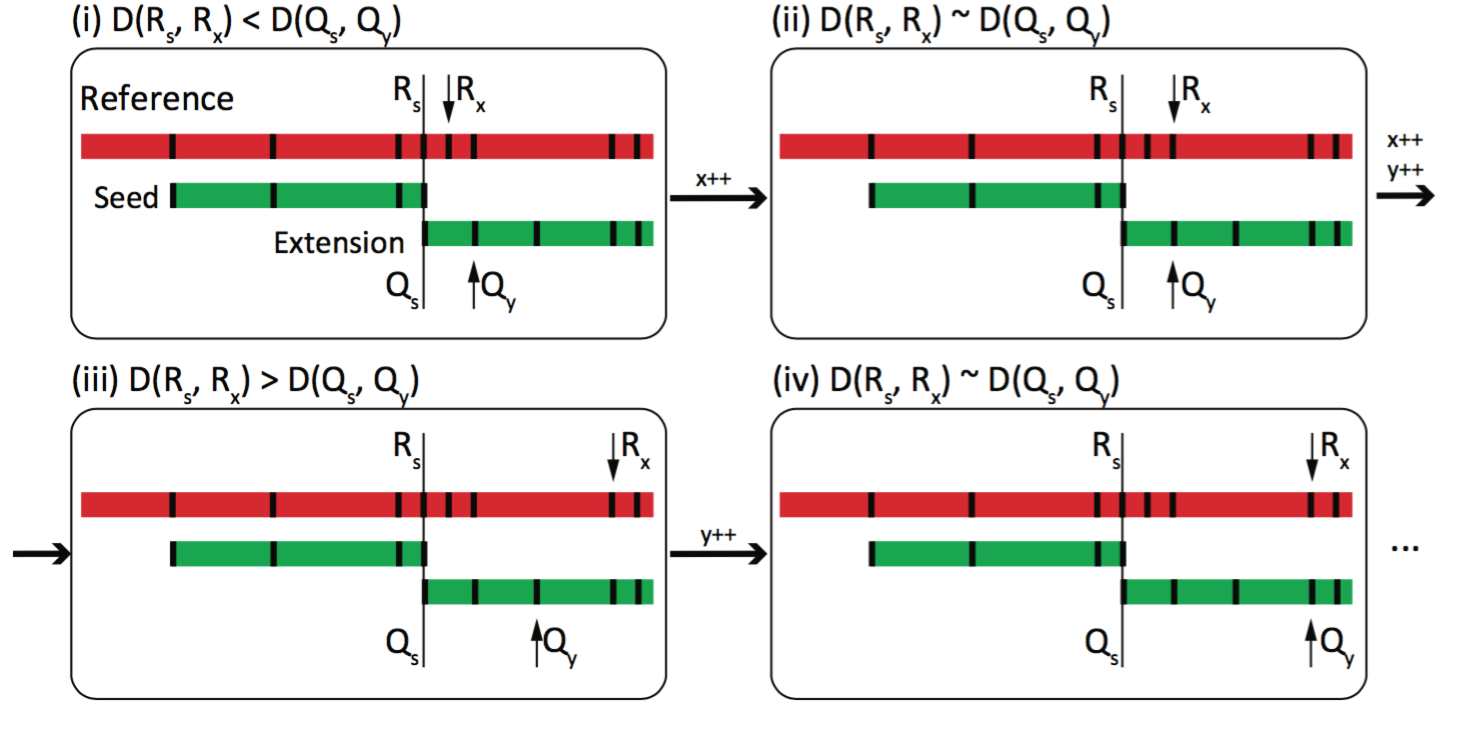
\includegraphics[width = 0.9\textwidth]{omblast/ext_seeds_2}
  \end{figure}
\end{frame}

\begin{frame}
\frametitle{OMBlast: Объединение выравниваний (1)}
  Строится взвешенный ациклический граф:
  \begin{itemize}
    \item Вершины - выравненные разрезы
    \item Рёбра - между двумя парами последовательно (на одной карте) выравненных разрезов
    \item Веса - $t_m \, u_m - t_{es} \, u_{es} - t_{ms} \, u_{ms}$ \\
    $u_{m}$ - количество совпадений\\
    $u_{es}$ - количество лишних разрезов\\
    $u_{ms}$ - количество пропущенных разрезов
  \end{itemize}
  \begin{figure}
    \centering
    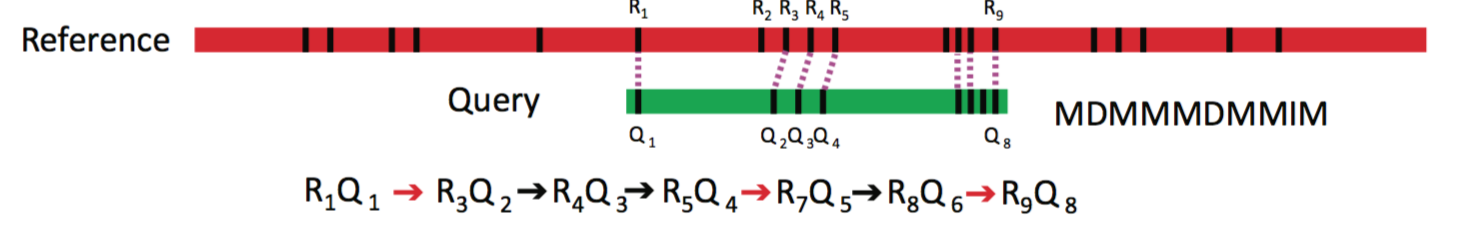
\includegraphics[width = 0.9\textwidth]{omblast/alg_mrg_0}
  \end{figure}
\end{frame}

\begin{frame}
\frametitle{OMBlast: Объединение выравниваний (2)}
  \begin{figure}
    \centering
    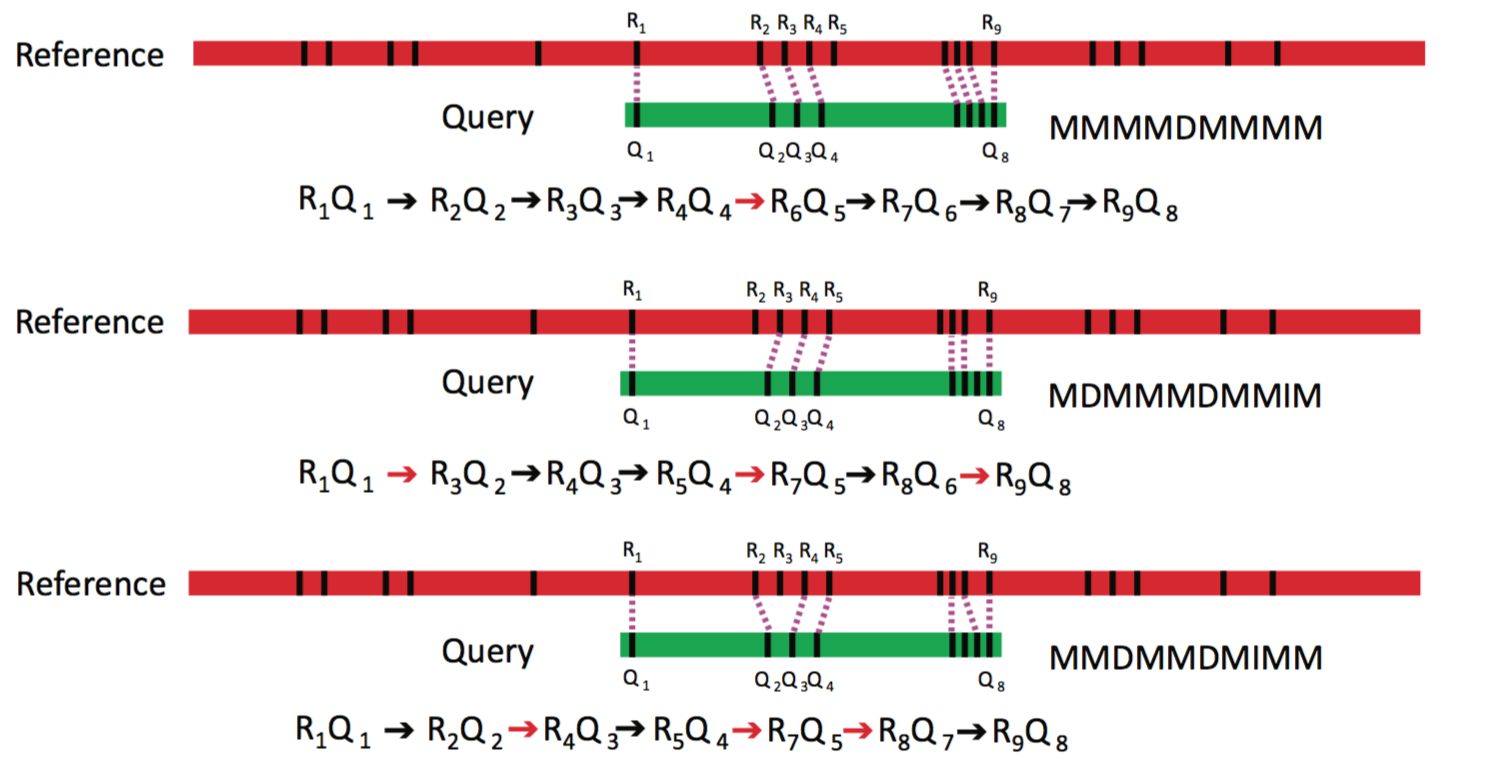
\includegraphics[width = 0.9\textwidth]{omblast/alg_mrg_2}
  \end{figure}
  \begin{figure}
    \centering
    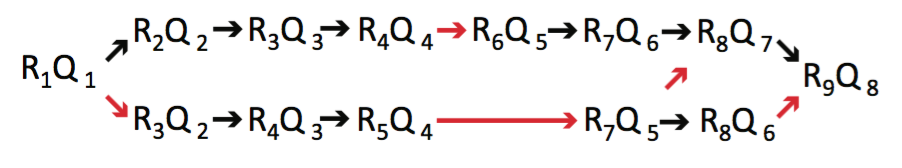
\includegraphics[width = 0.9\textwidth]{omblast/alg_mrg_3}
  \end{figure}

\end{frame}

\begin{frame}
\frametitle{OMBlast: Объединение выравниваний (3)}
С помощью динамического программирования определяется путь в графе с наибольшим весом
  \begin{figure}
    \centering
    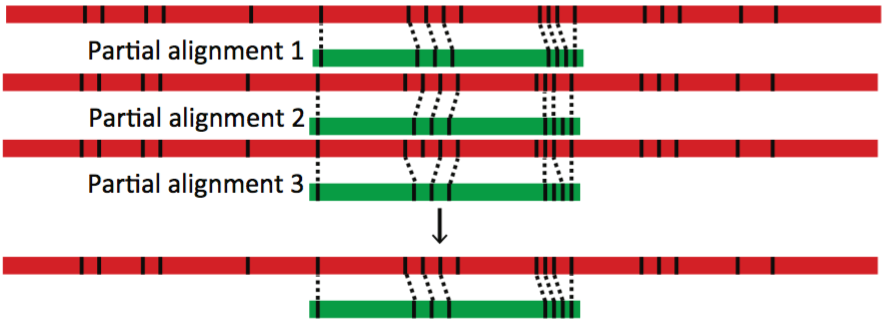
\includegraphics[width = 0.9\textwidth]{omblast/alg_mrg_1}
  \end{figure}

\end{frame}


\begin{frame}
\frametitle{OMBlast: Построение итогового выравнивания}


\end{frame}

\begin{frame}
\frametitle{OMBlast: Результаты - входные данные}
  \begin{figure}
    \centering
    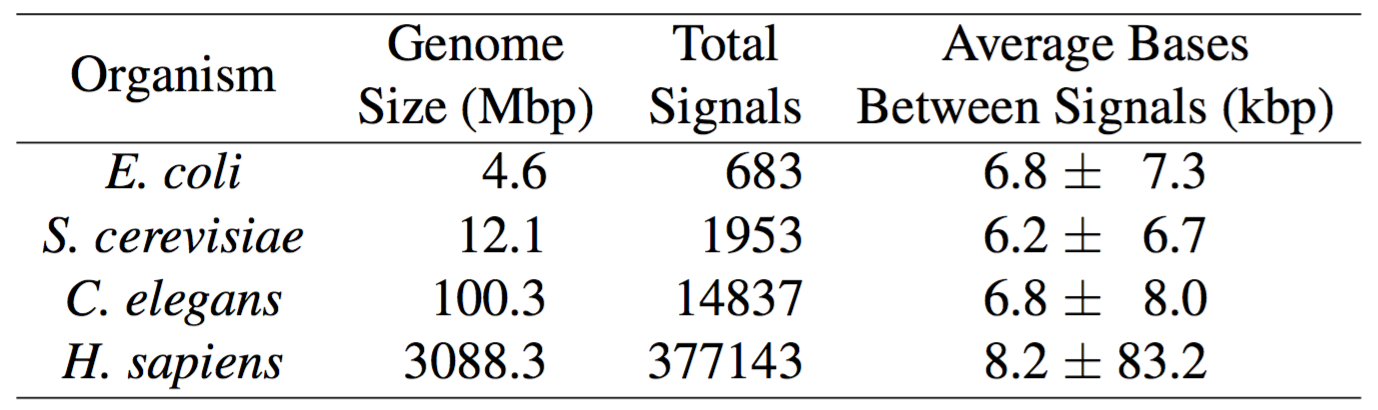
\includegraphics[width = 0.9\textwidth]{omblast/data}
  \end{figure}
  \begin{figure}
    \centering
    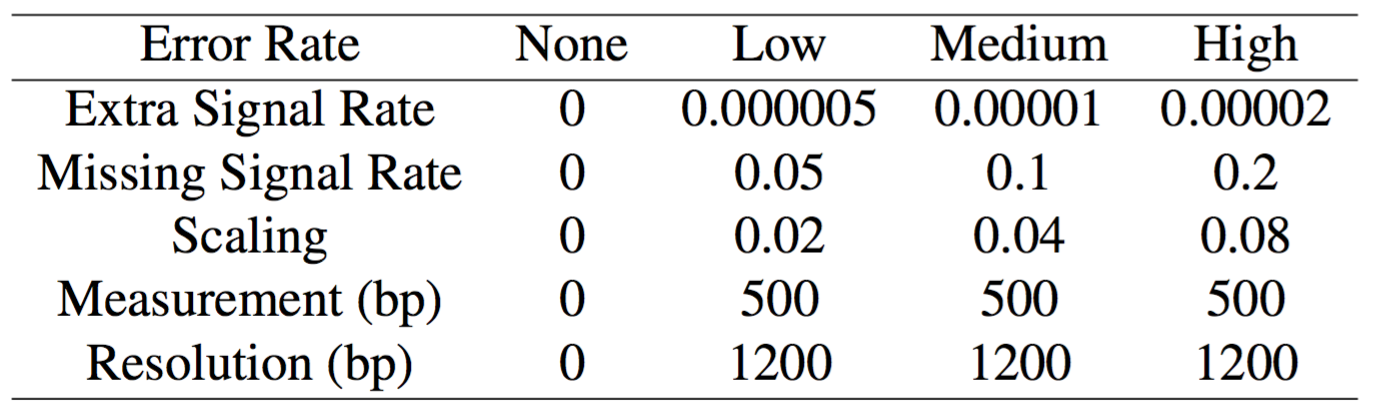
\includegraphics[width = 0.9\textwidth]{omblast/error_levels}
  \end{figure}
\end{frame}

\begin{frame}
\frametitle{OMBlast: Результаты - время работы}
  \begin{figure}
    \centering
    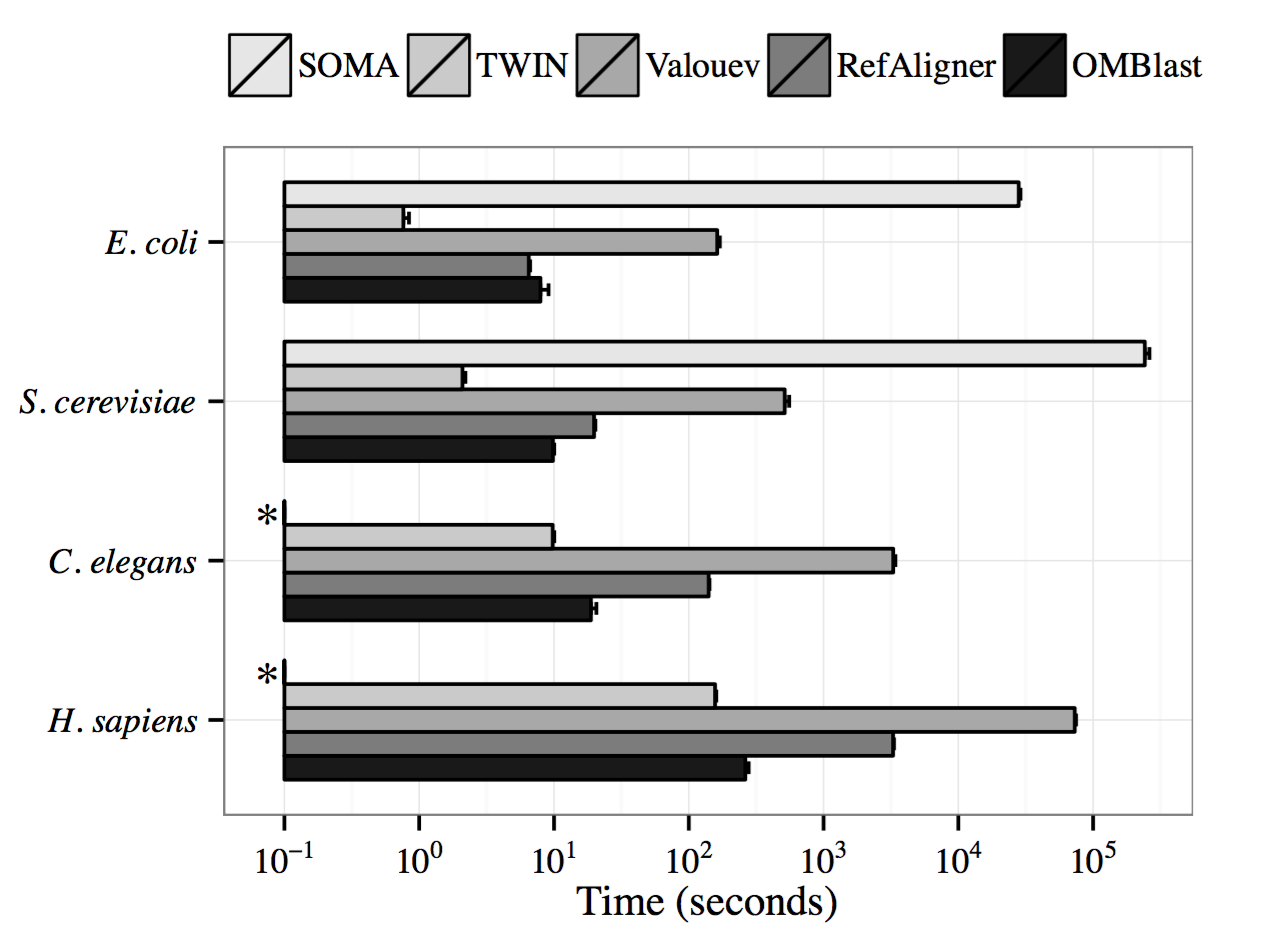
\includegraphics[width = 0.9\textwidth]{omblast/time}
  \end{figure}

\end{frame}

\begin{frame}
\frametitle{OMBlast: Результаты - точность и полнота }
  \begin{figure}
    \centering
    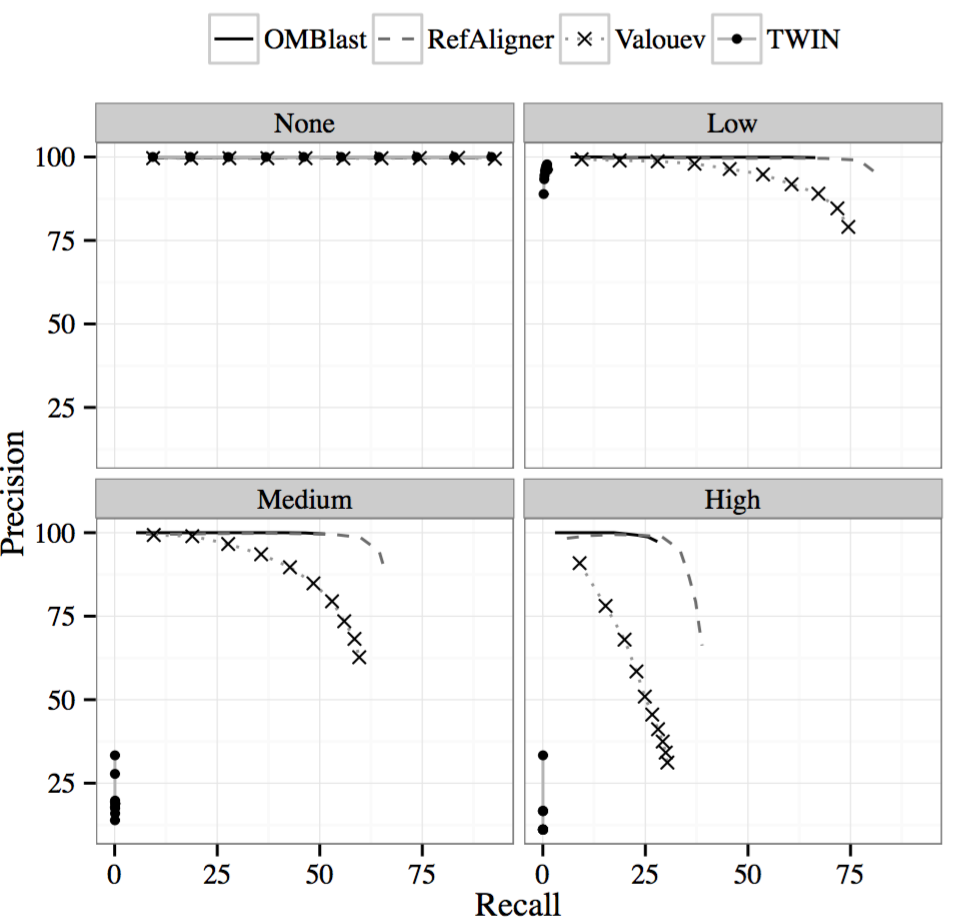
\includegraphics[width = 0.9\textwidth, height = 0.9\textheight]{omblast/error}
  \end{figure}

\end{frame}

\begin{frame}
\frametitle{OMBlast: Вывод }
Плюсы:
\begin{itemize}
  \item 
\end{itemize}
Минусы:
\begin{itemize}
  \item Предложенные схемы хешинга будут занимать много места
\end{itemize}
\end{frame}

% \begin{frame}
% \frametitle{OMBlast: Результаты - наличие SV}
%   \begin{figure}
%     \centering
%     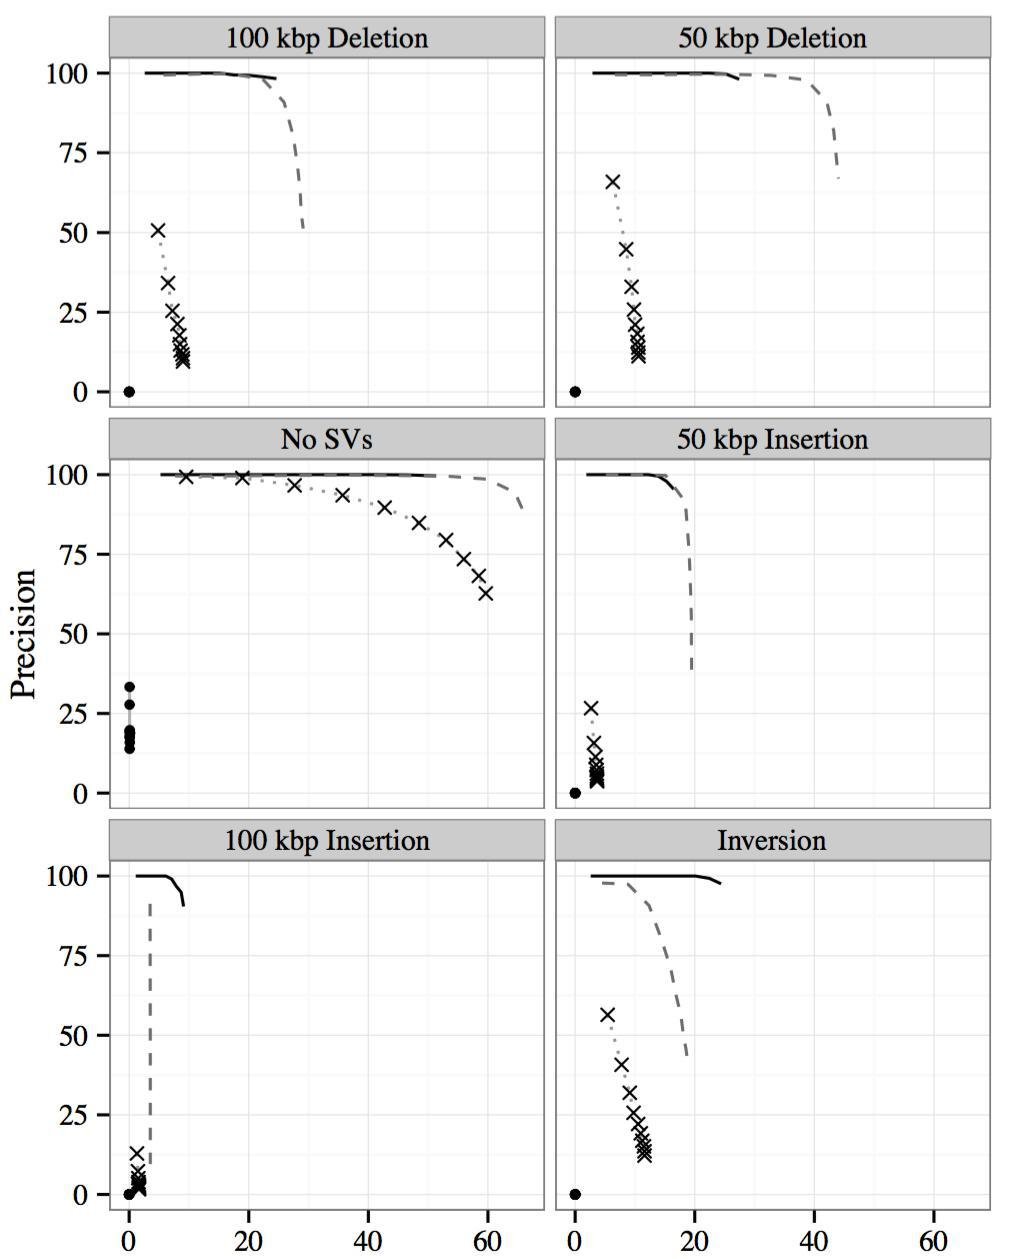
\includegraphics[width = 0.9\textwidth, height = 0.9\textheight]{omblast/sv}
%   \end{figure}
% \end{frame}


\section{Ссылки}
\begin{frame}
\frametitle{Ссылки: исходники}
В открытом доступе \nocite{*}:
\begin{itemize}
  \item \href{http://www.cs.colostate.edu/twin/download.html}{TWIN}
  \item \href{https://github.com/verznet/OPTIMA}{OPTIMA}
  \item \href{https://github.com/LeeMendelowitz/maligner}{MAligner}
  \item \href{https://github.com/aldenleung/OMBlast}{OMBlast}
\end{itemize}
\end{frame}

\begin{frame}[t,allowframebreaks]
\frametitle{Ссылки: статьи}
\printbibliography
\end{frame}

\begin{frame}

\begin{center}
\Huge Спасибо за внимание!
\end{center}

\end{frame}

\end{document}
